% !Mode:: "TeX:UTF-8"

\chapter{GAN}
\section{GAN Framework}

如下图所示,GAN包含一个用于产生的模型$G$,和一个用于判别的模型$D$。$G$和$D$是两个对抗的模型,$G$负责用来产生(采样)样本,$D$负责用来判断这个样本是由$G$产生的还是从数据集中抽样出来的。$D$尽可能的学习如何区分数据集中的样本和由$G$产生的样本,而$G$则尽可能的让产生的样本不被$D$区别开来。最终对抗的结果是,$D$学习到了数据集中所有样本的信息从而可以区分任何不是这个数据集中的样本,而$G$同样学习到了所有样本的信息,从而可以产生跟数据集完全一样的数据来让$D$混淆。

 \begin{figure}[htbp]
 \centering
 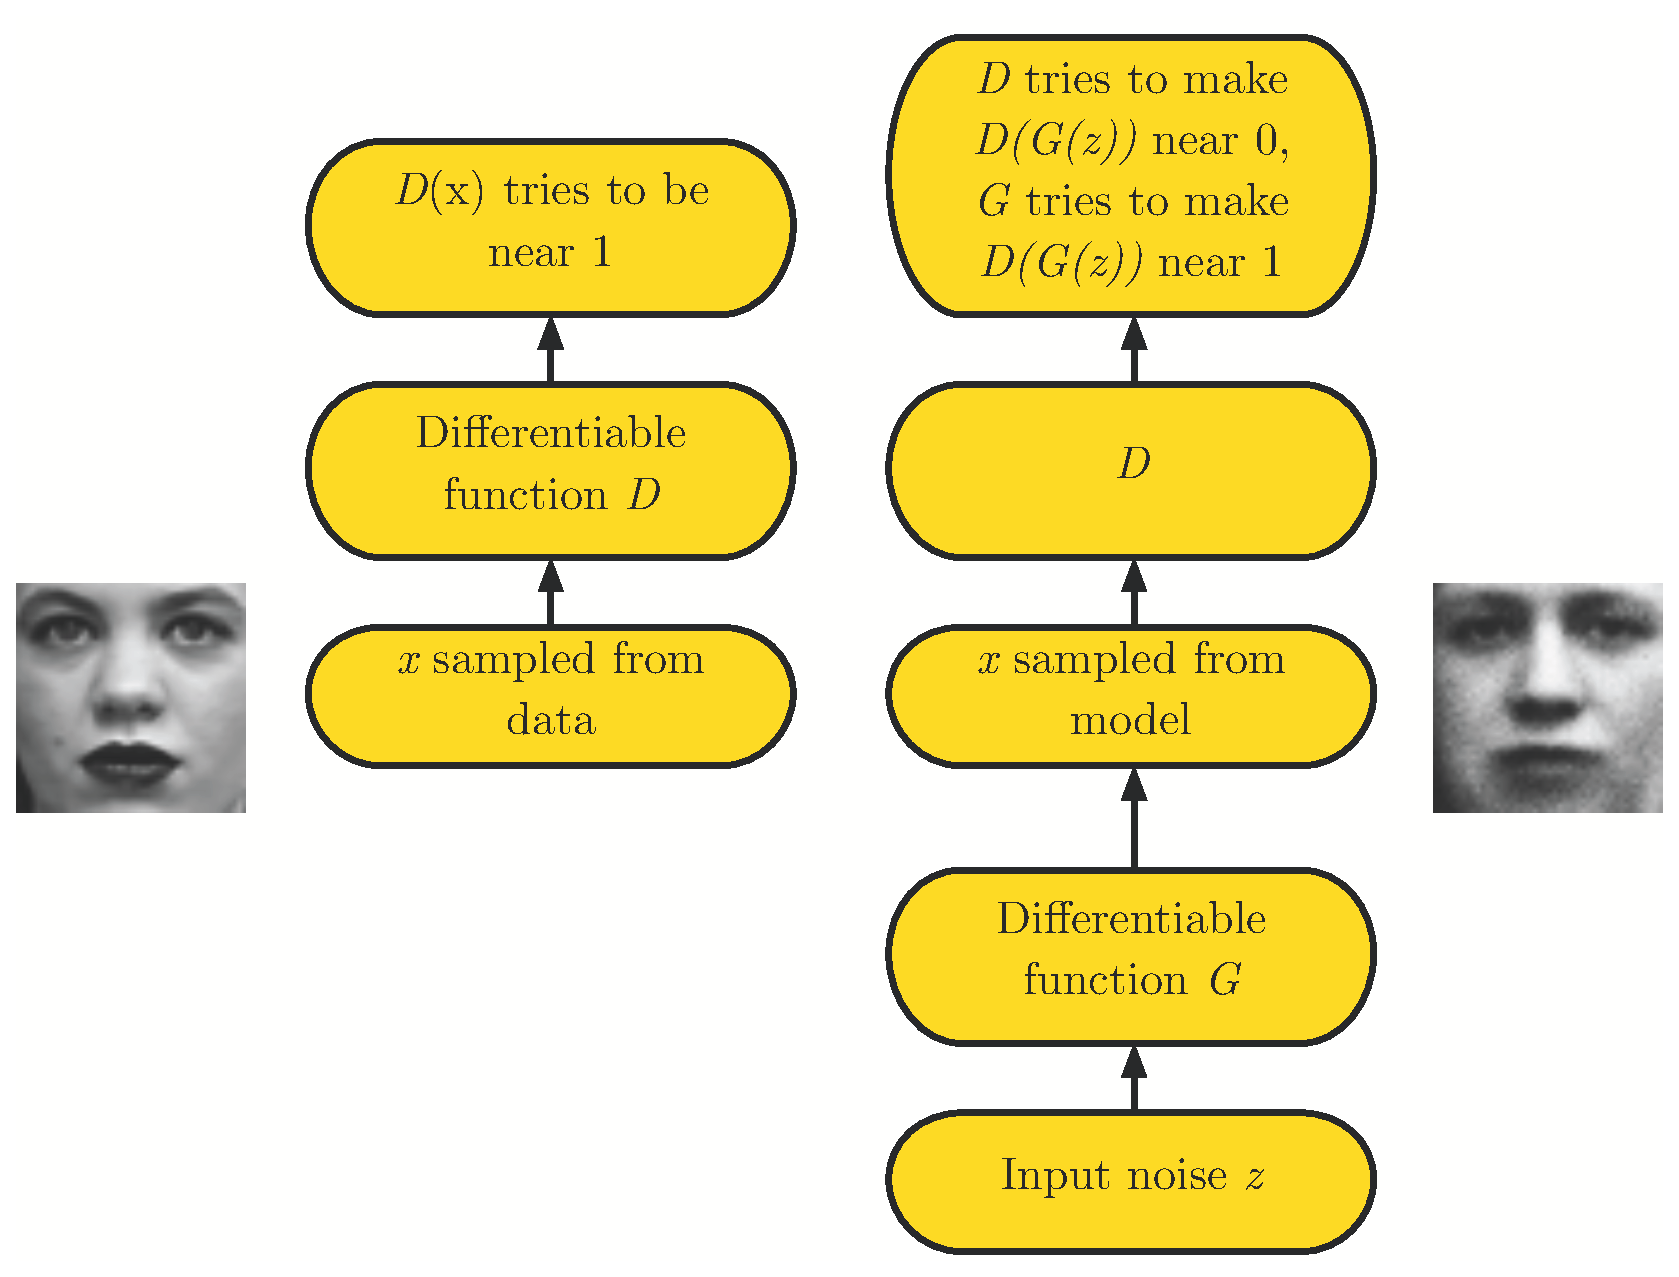
\includegraphics[width = 0.6\textwidth]{GAN_Framework}
 \end{figure}


由此我们可以得到GAN的优化目标如下,对模型$D$而言:
\begin{displaymath}
\mathbf{J}^{D}=-\frac{1}{2}\mathbb{E}_{{x}\sim p_{data}}\log{D({x})}-\frac{1}{2}\mathbb{E}_{{z}}\log(1-D(G({z}))))
\end{displaymath}
即,我们希望我们的模型$D$能够对数据集中所有的样本标记为1的概率最大,并对模型$G$产生的样本标记为0的概率最大。对模型$G$我们的优化目标正好同$D$相反,我们希望$G$产生的样本能够尽可能的让$D$标记为1,故而:
\begin{displaymath}
\mathbf{J}^{G}=\frac{1}{2}\mathbb{E}_{{z}}\log{(1-D(G({z})))}
\end{displaymath}

根据$\mathbf{J}^{D}$,我们求解$D(x)$如下:
\begin{displaymath}
\begin{split}
&\frac{\delta \mathbf{J}^{D}}{\delta D(x)} = \frac{\delta (-\frac{1}{2}\mathbb{E}_{{x}\sim p_{data}}\log{D({x})}-\frac{1}{2}\mathbb{E}_{{z}}\log(1-D(G({z}))))}{\delta D(x)} =0\\
&\mathbb{E}_{{x}\sim p_{data}}\log{D({x})} = \sum_{x}{p_{data}(x)\log{D(x)}}\\
&\mathbb{E}_{z}\log{(1-D(G(z)))} = \sum_{x}{p_{model}(x)\log{(1-D(x))}}\\
&\sum_{x}{\frac{p_{data}(x)}{D(x)} - \frac{p_{model}(x)}{1-D(x)}} = 0\\
&D(x) = \frac{p_{data}(x)}{p_{data}(x) + p_{model}(x)}\\
\end{split}
\end{displaymath}

GAN的训练算法如下:

\begin{figure}[htbp]
\centering
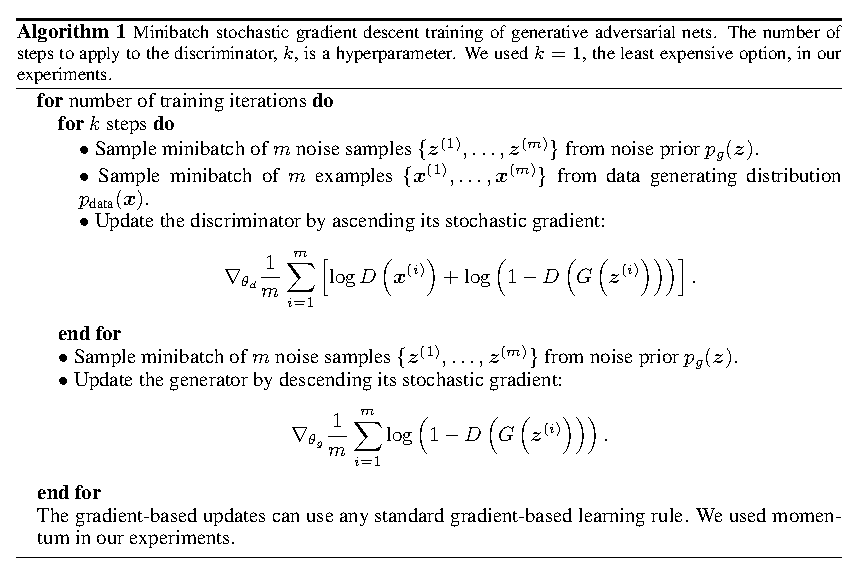
\includegraphics[width = 0.9\textwidth]{GAN_Train}
\end{figure}


下图是训练过程的一个形象化的演示:黑色虚线表示了数据的真实分布$\hat{G}$(未知的,我们只知道数据本身),绿色实线表示初始的$G$,蓝色虚线表示初始的$D$。初始的$G$同数据的真实分布$\hat{G}$差别较大,并不能很好的拟合数据,而初始的$D$也不能对一个样本是来自数据还是来自$G$做出很好的判别。我们固定$G$来训练$D$之后,$D$能够对区分$\hat{G}$和$G$,我们进一步的固定$D$来训练$G$使得$G$更接近$\hat{G}$,从而迷惑$D$。重复这个过程之后$G$将会尽可能的接近$\hat{G}$,而$D$会不能区分$G$和$\hat{G}$。
\begin{figure}[htbp]
\centering
\includegraphics[width = 1.0\textwidth]{GAN_UpdateDG}
\end{figure}

令$P_r$为真实数据的分布,$P_g$为生成器的数据分布,则生成器的算是可以写为:$\mathbb{E}_{x \sim P_g}[\log (1- D(x))]$。我们将该损失添加一个不依赖于生成器的一项,变为:$\mathbb{E}_{x \sim P_r}[\log (D(x))] + \mathbb{E}_{x \sim P_g}[\log (1- D(x))]$,并将$D(x) = \frac{P_{r}(x)}{P_{r}(x) + P_{g}(x)}$带入得:

\begin{displaymath}
\begin{split}
&\mathbb{E}_{x \sim P_r}[\log (D(x))] + \mathbb{E}_{x \sim P_g}[\log (1- D(x))] \\
&= \mathbb{E}_{x \sim P_r}[\log (\frac{P_{r}(x)}{P_{r}(x) + P_{g}(x)})] + \mathbb{E}_{x \sim P_g}[\log (1- \frac{P_{r}(x)}{P_{r}(x) + P_{g}(x)})] \\
&= \mathbb{E}_{x \sim P_r}[\log (\frac{P_{r}(x)}{P_{r}(x) + P_{g}(x)})] + \mathbb{E}_{x \sim P_g}[\log (\frac{P_{g}(x)}{P_{r}(x) + P_{g}(x)})] \\
&= \mathbb{E}_{x \sim P_r}[\log (\frac{P_{r}(x)}{\frac{1}{2}(P_{r}(x) + P_{g}(x))})] + \mathbb{E}_{x \sim P_g}[\log (\frac{P_{g}(x)}{\frac{1}{2}(P_{r}(x) + P_{g}(x))})] -2 \log 2 \\
&= 2 JS(P_r, P_g) - 2log2\\
\end{split}
\end{displaymath}

即生成器的训练实际上是最小化真是数据分布$P_r$和模型数据分布$P_g$的JS距离。

\section{非饱和GAN}
当我们使用:$\mathbb{E}_{x \sim P_g}[\log (1- D(x))]$作为生成器的损失时会存在一个问题,就是在训练G时,我们最小化$JS(P_r, P_g)$,而在训练D时,我们最大化$JS(P_r, P_g)$。当判别器D以非常高的置信度拒绝一个样本时,产生器G的梯度就会消失。为了解决这个问题,我们可以将产生器的损失变换为$-\mathbb{E}_{x \sim P_g}[\log (D(x))]$。

\begin{displaymath}
\begin{split}
KL(P_g \parallel P_r) &= \mathbb{E}_{x \sim P_g} [\log \frac{P_g(x)}{P_r(x)}]\\
&= \mathbb{E}_{x \sim P_g} [\log \frac{P_g(x)/(P_r(x) + P_g(x))}{P_r(x)/(P_r(x) + P_g(x))}]\\
&= \mathbb{E}_{x \sim P_g} [\log \frac{1-D(x)}{D(x)}]\\
&= \mathbb{E}_{x \sim P_g} [\log {1-D(x)}] -\mathbb{E}_{x \sim P_g} [\log {D(x)}]\\
\mathbb{E}_{x \sim P_r}[\log (D(x))] + \mathbb{E}_{x \sim P_g}[\log (1- D(x))] &= 2 JS(P_r, P_g) - 2log2\\
-\mathbb{E}_{x \sim P_g}[\log (D(x))] &= KL(P_g \parallel P_r) - 2 JS(P_r, P_g) + 2log2 + \mathbb{E}_{x \sim P_r} [\log {D(x)}]\\
\end{split}
\end{displaymath}

则训练产生器G的优化目标$-\mathbb{E}_{x \sim P_g}[\log (D(x))]$,转换为$KL(P_g \parallel P_r) - 2 JS(P_r, P_g)$(公式中最后两项与G无关)。这样的一个优化目标是有问题的,它同时要求最小化$P_g$和$P_r$的KL距离,而又最大化两者的JS距离,在数值上会导致梯度非常的不稳定。另一方面由于KL距离是一个非对称的距离,这会导致
\begin{itemize}
\item 当$P_g(x) \to 0$而$P_r(x) \to 1$时,KL距离为0,
\item 当$P_g(x) \to 1$而$P_r(x) \to 0$时,KL距离为无穷大,
\end{itemize}
也就是说,当生成器没能够生成真实样本时,惩罚比较小,但当生成器生成了一个不真实的样本时,惩罚非常大。这样子训练出来的模型就会宁愿多生成一个重复而保险的样本,也不会冒险生成多样性的样本,这就是mode collapse问题。

\section{WGAN}
\subsection{不同的距离函数}
令 $\mathcal{X}$为紧矩阵空间(比如$[0,1]^d$),$\Sigma$为该空间的所有Borel子集的集合,$Prob(\mathcal{X})$为定义在$\mathcal{X}$上的概率分布的空间,对于任意的两个概率分布$\mathbb{P}_r, \mathbb{P}_g \in Prob(\mathcal{X})$,我们可以有如下的几个距离函数:

\textbf{Total Variantion(TV) Distance}: $\delta{({P}_r, {P}_g)} = \underset{A \in \Sigma}{sup} \left | {P}_r(A) -{P}_g(A) \right |$。 TV距离试图在定义域$\mathcal{X}$上寻找一个子集$A$,使得在该子集上两个概率分布的差最大。该最大的差即为TV距离。

\textbf{Kullback-Leibler(KL) Distance}: $KL({P}_r \parallel {P}_g) = \int \log (\frac{P_r(x)}{P_g(x)})P_r(x) \mathrm{d} \mu(x) $,其中$\mu(x)$为定义在$\mathcal{X}$上的测度。KL距离是非对称的,并且当$P_g{x} = 0$并且$P_r(x) > 0$时,其距离为无穷大。

\textbf{Jensen-Shannon(JS) Distance}:$JS({P}_r, {P}_g) = \frac{1}{2}KL({P}_r \parallel {P}_m) + \frac{1}{2}KL({P}_g \parallel {P}_m)$,其中${P}_m = \frac{\mathbb{P}_r + \mathbb{P}_g}{2}$。JS距离是对称的,{\color{red} 如果其中的$KL$距离的$\mu = \mathbb{P}_m$,则JS距离则在空间$\mathcal{X}$上永远有定义}。

\textbf{Earth Mover(EM) Distance}:$W({P}_r,{P}_g) = \underset{\gamma \in \Pi({P}_r, {P}_g)}{inf} \mathbb{E}_{(x,y) \sim \gamma} [\left \| x-y \right \|]$. 其中,$\gamma(x,y)$是以 $\mathbb{P}_r(x)$和$\mathbb{P}_g(x)$为边缘分布的$(x,y)$的联合分布, $\Pi({P}_r, {P}_g)$为所有$\gamma$的集合。对于一个可能的联合分布$\gamma$,我们可以采样一个$(x,y)$,并计算其距离$\left \| x-y \right \|$。对于分布$\gamma$,我们便可以计算在该分布下,距离$\left \| x-y \right \|$的期望值。在所有的可能的联合分布$\gamma$中,我们可以找到一个分布使得该距离的期望最小,这个最小的期望,便是EM距离。直觉上,如果我们把$\mathbb{P}_r$和$\mathbb{P}_g$看作在定义域上两种不同方式堆积的土堆,并$\gamma(x,y)$定义了如何将土堆${P}_r$变为${P}_g$的移动方式,那么EM距离就是将${P}_r$转变为${P}_g$的所有需要移动的单位小块的最小距离之和。

\textbf{平行线例子}: 我们令$Z \sim U[0,1]$,并令${P}_0$为$(0, Z) \in {R}^2$的分布,该分布在x轴上只在点0处有密度,而在y轴上在$[0,1]$区间上均匀分布。类似的,我们令${P}_\theta$为$(\theta, Z) \in \mathbb{R}^2$的分布,该分布在x轴上只在点$\theta$处有密度,而在y轴上在$[0,1]$区间上均匀布分布。那么分布${P}_0$和分布${P}_\theta$的距离为:
\begin{displaymath}
\begin{split}
\delta({P}_0, {P}_\theta) &= 
\begin{cases}  
1 ~~~ if ~~\theta \neq 0\\
0 ~~~ if ~~ \theta = 0\\
\end{cases}\\
KL({P}_0 \parallel {P}_\theta) &= KL({P}_\theta \parallel {P}_0) = 
\begin{cases}  
+ \infty ~~~ if ~~\theta \neq 0\\
0 ~~~ if ~~ \theta = 0\\
\end{cases}\\
JS({P}_0, {P}_\theta) &= 
\begin{cases}  
\log 2 ~~~ if ~~\theta \neq 0\\
0 ~~~ if ~~ \theta = 0\\
\end{cases}\\
W({P}_0, {P}_\theta) &= |\theta|\\
\end{split}
\end{displaymath}

对于TV距离,很明显,我们选定义域$\mathcal{X}$的一个子集$(0, [0,1])$, ${P}_0$在该子集上概率为1, ${P}_\theta$在该子集上概率为0,且其差为最大。

对于KL距离:
\begin{displaymath}
\begin{split}
KL({P}_0 \parallel {P}_\theta) &= \int_{0}^{1} \log (\frac{P_0(0,x)}{P_\theta(0,x)})P_0(0,x) \mathrm{d} x + \int_{0}^{1} \log (\frac{P_0(\theta,x)}{P_\theta(\theta,x)})P_0(\theta,x) \mathrm{d} x
\end{split}
\end{displaymath}
很明显当$\theta =0$时,其值为0, 当$\theta \neq 0$时,在子空间$(0,[0,1])$上积分为$+\infty$,在子空间$(\theta, [0,1]$上积分为0,故,距离为$+\infty$。同样的$KL({P}_\theta \parallel {P}_0)$也是如此。

对JS距离, 当$\theta =0 $时,很明显距离为0, 当$\theta \neq 0$时,:
\begin{displaymath}
\begin{split}
2JS({P}_0 \parallel {P}_\theta) 
&= KL({P}_0 \parallel \frac{{P}_0 + {P}_\theta}{2}) + KL({P}_\theta \parallel \frac{{P}_0 + {P}_\theta}{2}) \\
&= \int_{0}^{1} \log (\frac{P_0(0,x)}{\frac{P_0(0,x) + P_\theta(0,x)}{2}})P_0(0,x) \mathrm{d} x +
   \int_{0}^{1} \log (\frac{P_0(\theta,x)}{\frac{P_0(\theta,x) + P_\theta(\theta,x)}{2}})P_0(\theta,x) \mathrm{d} x\\
&+ \int_{0}^{1} \log (\frac{P_\theta(0,x)}{\frac{P_0(0,x) + P_\theta(0,x)}{2}})P_\theta(0,x) \mathrm{d} x +
   \int_{0}^{1} \log (\frac{P_\theta(\theta,x)}{\frac{P_0(\theta,x) + P_\theta(\theta,x)}{2}})P_\theta(\theta,x) \mathrm{d} x\\
&= \int_{0}^{1} \log (\frac{P_0(0,x)}{\frac{P_0(0,x)}{2}})P_0(0,x) \mathrm{d} x +
   \int_{0}^{1} \log (\frac{0}{\frac{P_\theta(\theta,x)}{2}})*0 \mathrm{d} x\\
&+ \int_{0}^{1} \log (\frac{0}{\frac{P_0(0,x)}{2}}) *0 \mathrm{d} x +
   \int_{0}^{1} \log (\frac{P_\theta(\theta,x)}{\frac{P_\theta(\theta,x)}{2}})P_\theta(\theta,x) \mathrm{d} x\\
&=  \int_{0}^{1} \log (2)P_0(0,x) \mathrm{d} x + \int_{0}^{1} \log (2)P_\theta(\theta,x) \mathrm{d} x\\
&= 2 \log 2\\
JS({P}_0 \parallel {P}_\theta) &= \log 2\\
\end{split}
\end{displaymath}

对EM距离,我们选择以 ${P}_0(x)$和${P}_\theta(x)$为边缘分布的$(x,y)$的联合分布$\gamma(x,y)$为定义域为$(0, \theta, x, y)$上的分布,其中$x,y \in [0,1]$,则,在该分布下,距离的期望为:
\begin{displaymath}
\begin{split}
&\int_0^1 \int_0^1 p_{\gamma}(0,\theta,x, x) \left \| (0,x) - (\theta, x) \right \| \mathrm{d} x  \mathrm{d} y \\
&= \int_0^1 \int_0^1 p_{\gamma}(0,\theta,x, x)  \left \| (0,x) - (\theta, y) \right \| \mathrm{d} x   \mathrm{d} y\\
&= \int_0^1 \int_0^1 p_{\gamma}(0,\theta,x, x)  \sqrt {\theta ^ 2 + (x-y)^2}\mathrm{d} x \mathrm{d} y\\
& \leq \int_0^1 \int_0^1 p_{\gamma}(0,\theta,x, x) |\theta| \mathrm{d} x \mathrm{d} y\\
&= |\theta|\\
\end{split}
\end{displaymath}
不等式等号成立的条件是联合分布$\gamma(x,y)$为定义域为线段$(0, \theta, x, y=x)$上的均匀分布。

由上可知,当${P}_r$和${P}_g$没有重叠的时候,TV,KL, JS距离均为不连续函数,其导数为0。
更一般的,给定高维空间的两个分布${P}_r$和${P}_g$,当他们的支撑集是高维空间的低维流形时, ${P}_r$和${P}_g$重叠部分测度为0的概率为1。

对GAN的产生器来说,输入为一个低维的向量,产生一个高维的样本,其支撑集便是高维空间的低维流形。故而,GAN的产生器${P}_g$和真实分布${P}_r$几乎没有重叠的可能。故而当使用TV/KL/JS距离作为损失时,导数为0。

\subsection{WGAN}

由前边我们知道EM距离相比TV, KL, JS更适合来做GAN的loss function。然而当我们试图使用EM距离来取代KL/JS距离时,存在一个问题,因为EM距离里边需要计算所有可能联合分布的一个下界。$W({P}_r,{P}_g) = \underset{\gamma \in \Pi({P}_r, {P}_g)}{inf} \mathbb{E}_{(x,y) \sim \gamma} [\left \| x-y \right \|]$。我们可以使用Kantorovich-Rubinstein duality来将EM距离改写为:

\begin{displaymath}
\begin{split}
W({P}_r, {P}_g) & = \underset{\left \| f \right \|_{L} \leq 1}{sup} \mathbb{E} _{X \sim {P}_r}[f(x)] - \mathbb{E}_{x \sim {P}_g}[f(x)]
\end{split}
\end{displaymath}
其中 $ \underset{\left \| f \right \|_{L} \leq 1}{sup} $表示在所有的符合1-Lipschitz连续的函数中,寻找一个令$\mathbb{E} _{X \sim {P}_r}[f(x)] - \mathbb{E}_{x \sim {P}_g}[f(x)]$最大的上界。

那么什么是Lipschitz连续? Lipschitz连续是一个比连续更强的光滑性的条件。Lipschitz连续函数限制了函数改变的速度,函数的斜率必须小于一个Lipschitz常数的实数。设$d_X$和$d_Y$分别为$X$和$Y$空间的两个度量,函数$f:X \to Y$是K-Lipschitz连续的当且仅当对于任意的$x_1, x_2 \in X$, 有 $d_Y(f(x_1), f(x_2)) \leq K d_X(x_1, x_2)$。

我们进一步的将所有满足1-Lipschitz连续的函数约束在一个以$w \in \mathcal{W}$($\mathcal{W}$为参数空间)为参数的函数$f_w$的子空间里,则:

\begin{displaymath}
\begin{split}
W({P}_r, {P}_g) & = \underset{\left \| f \right \|_{L} \leq 1}{sup} \mathbb{E} _{X \sim {P}_r}[f(x)] - \mathbb{E}_{x \sim {P}_g}[f(x)]\\
& \ge \underset{w \in \mathcal{W}}{max} \mathbb{E} _{X \sim {P}_r}[f_w(x)] - \mathbb{E}_{x \sim {P}_g}[f_w(x)]\\
\end{split}
\end{displaymath}

当我们需要训练一个$P_g = g_\theta(Z)$来拟合$P_r$时,我们首先要训练一个$f_w$来计算EM距离,然后基于这个EM距离来优化$g_\theta$,具体的:
\begin{itemize}
\item 给定$\theta$,训练$f_w$收敛以获得EM距离 $W(P_r, P_g)$的一个近似。
\item 给定优化的$f_w$,采样若干的$z \sim Z$,并计算$\theta$的梯度:$\nabla_\theta W(P_r, P_g) = \nabla_\theta(\mathbb{E}_{x \sim P_r}[f_w(x)] - \mathbb{E}_{z \sim Z}[f_w(g_\theta(z))]) = -\mathbb{E}_{z \sim Z}[f_w(g_\theta(z))]) $.
\item 更新$\theta$,并重复步骤1.
\end{itemize} 

具体的WGAN的训练过程为:

 \begin{figure}[htbp]
 \centering
 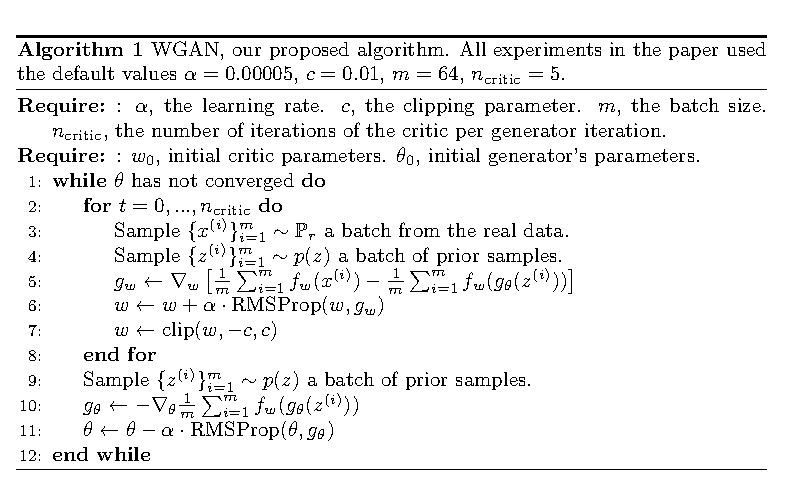
\includegraphics[width = 0.9\textwidth]{WGAN}
 \end{figure}

同原始的GAN相比,WGAN有如下几点改动:
\begin{itemize}
\item 判别器最后一层去调sigmoid,即已经不能做分类,可以看作一个critic
\item 生成器和判别器的loss不取log,因为仅仅是一个Lipschitz连续的函数,已经不是概率,有可能为负。
\item 每次更新判别器的参数之后,绝对值要截断到不超过常数$c$,以保证更新完之后仍然是一个Lipschitz连续的函数。
\item 不要使用基于动量的优化算法(Momentum和Adam),推荐RMSProp和SGD。 
\end{itemize} 


\section{DCGAN}

\section{SeqGAN}